\chapter{Convolutional Neural Network}
\textbf{CNNs} are particular types of neural network feed forward. Their goal 
is to use multiple layers, stacked one on top of the other, in order to 
extract input-related features. These stages are organized in a hierarchical 
way, where the highest level calculates more global, more invariant features.

Unlike the networks seen so far, CNNs organize weights using 3 dimensions. From 
this point on, we will talk about the weights also considering the volume. We are 
talking of volumes because we have image width different number of channel in input,
each neuron applies as filter on all spatial dimensions and all channel. In output 
of each layer we have another volume with a deph dependant by the number of neuorns
of hidden layer. 


\begin{figure}[!ht]
    \centering
    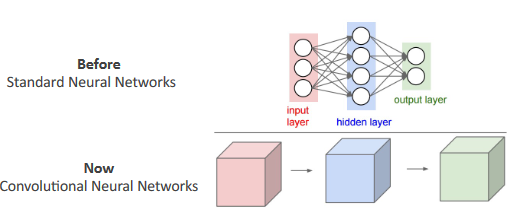
\includegraphics[width=0.5\textwidth]{img/CNN/weights.png}
    \caption{Weights representation in Feed Forward vs CNN.}
    \label{fig:weights}
\end{figure}

This particular type of network is widely used in the field of digital signal 
processing, such as image or audio signals. If we look at image processing, this 
kind of neural network offers a much more cost-effective approach than traditional 
feed forward. 

The biggest difference is related to the fact that in a feed network farward each 
input neuron is connected to all the neuorns of the next layer, this results in a 
big problem at the level of complexity, If we have an image of $100 \times 100$ pixels, 
for example, the network input is a vector of $10000$ pixels. Using CNNs means that 
each neuron is focused on a small portion of the image for each channel (\textbf{Local connectivity}) 
so that the number of neurons and connections that are created is greatly reduced.
If the image is a $1000\times 1000\times 3$, so we can have a neuron of $5\times 5 \times 3$
parameter because it applies to a path of $5\times 5$ for each deaph of the layer 
before (\textbf{full in depth}). 

\begin{figure}[!ht]
    \centering
    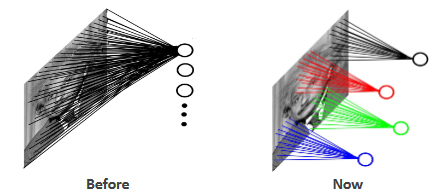
\includegraphics[width=0.5\linewidth]{img/CNN/localConn.png}
    \caption{Difference between the connections of neurons in a feed forward network and a CNN.}
    \label{fig:localConn}
\end{figure}

Also, another difference is that now, we have neurons organized in depth, we have 
multiple neurons all looking the same region of the input volume, stacked along depth.

\begin{figure}[!ht]
    \centering
    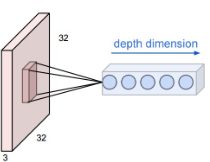
\includegraphics[width=0.25\linewidth]{img/CNN/depth.png}
    \caption{Organization of neurons in CNN}
    \label{fig:depth}
\end{figure}

In total we have $5\times 5\times 3$ weights to Learn
shared between each patch of the image, this reduce a lot the number of learning 
parameter compared to FF.  
This concept is called \textbf{weights sharing}, which means that the weights 
in the layer are shared across spatial positions. 

In general, the structure of a CNN is organized so that it has a first part, which 
includes both convolutional layers and feed forward layers, extract the main 
characteristics from the input. There is then a second part which performs the actual
classification task. We can then represent this type of network with a structure like 
the one shown in figure \ref{fig:cnn-arc}.

\begin{figure}[!ht]
    \centering
    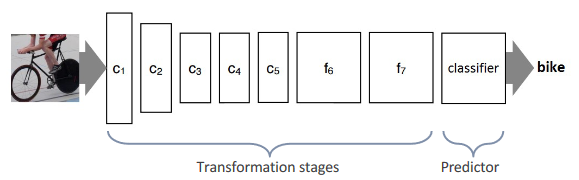
\includegraphics[width=\linewidth]{img/CNN/CNNarc.png}
    \caption{Overall CNN architecture.}
    \label{fig:cnn-arc}
\end{figure}

The concept of backpropagation can still be utilized with this architecture, which is 
very important.

Respect to traditional Neural Networks, CNNs have other special layers such as \textbf{Spatial pooling} and \textbf{Local response normalization}. These layers are 
useful to reduce computational burden, increase invariance and ease the optimization.
\section{CNNs components}
\subsection{Linear Convolution}
We begin by introducing the concept behind convolutional networks, namely the concept 
of \textbf{linear convolution}. Convolution is a linear (the operation is linear), 
local (it applies on patches) and translation-invariant
operator. If you want a richer representation of the data, you use a \textbf{filter bank},
that is a collection of $Q$ sets of $K$ filters that allows to produce an output of 
$Q$ channel.

Let's see now, on a more mathematical level, what convolution represents. First we 
introduce what we need:
\begin{itemize}
    \item $x = H \times W \times K$ is our input where $H$ represents the height dimension, $W$ the width dimension and $K$ the number of channels.
    \item $F = H' \times W' \times K \times Q$ is our filter bank where $Q$ is the number of filters that need to be apply to each channel.
    \item $y = (H - H' + 1) \times (W - W' + 1) \times Q$ is our output.
\end{itemize}

In addition to these, another very important thing to define is the \textbf{stride}. 
It represents how much I have to move my filter before I can apply it again. By default 
it is set to 1, which means I only move the center of my filter one pixel. 

The convolution is expressed by the following formula:
\begin{equation}
    y_{i, j, q} = y_q + \sum_{u = 0}^{H - 1}\sum_{v = 0}^{W - 1}\sum_{k = 1}^{K} x_{u + i, v + j, k} \cdot F_{u, v, k, q} 
\end{equation}

where:
\begin{itemize}
    \item $y_q$ is the bias of the filter $F_q$
    \item $x_{u + i, v + j, k}$ is the input patch of channel $k$
    \item $F_{u, v, k, q}$ is the filter for the channel $k$ that computes output channel $q$ 
\end{itemize}

\begin{figure}[!ht]
    \centering
    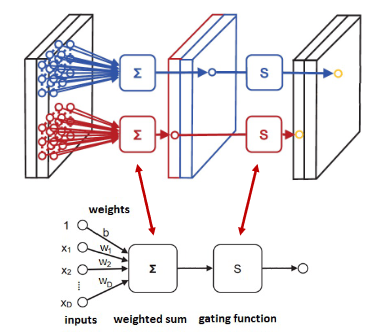
\includegraphics[width=0.5\linewidth]{img/CNN/Conv2Filter.png}
    \caption{Example of convolutional network with a filter bank of two elements.}
    \label{fig:conv2filter}
\end{figure}

We can apply filters in 2 way:
\begin{itemize}
    \item \textbf{lattice structure}: a single filter is applied to a single channel  $K=1$
    \item \textbf{multiple feature structure}: a single filter is applied to all 
    channel of the input image.$K>1$
\end{itemize}

In CNN, after appling filter we apply non linear activation function:
\begin{itemize}
    \item sigmoid
    \item tanh
    \item ReLU
    \item SmoothReLU
\end{itemize}  
activation function are called \textbf{gating function}.

\subsection{Spatial pooling}
We have already said that there are different types of layers in a CNN, one of them is 
the \textbf{spatial pooling}. This layer is intended to subsample the image in order 
to reduce the spatial scale and consequently the computation, but also to aggregate 
it to obtain the translation invariance obtaining robustness to the exact spatial 
localization of the characteristics. This is done in two main ways: 
\begin{itemize}
    \item \textbf{avg pooling}: averaging the nearest 
    pixels
    $$y_{ijk} =\max \limits_p,q\in \Omega x_{pqk}$$
    \item \textbf{max pooling}: taking the maximum value from the nearest ones
    $$y_{ijk} =\text{avg}_p,q\in \Omega x_{pqk}$$
\end{itemize}

This is done channel by channel.
\subsection{Local Response Normalization}
\textbf{Local Response Normalization} layers have the objective of normalizing the 
effect of contrast to improve the network invariance in this respect. This layer 
also allows for improved optimization and sparsity.

In general, there are two ways of applying it:
\begin{itemize}
    \item \textbf{Within Channel}: operates independently on different feature channels, and also rescales each input feature basing on a local neighborhood.
    \begin{equation}
        y_{i, j, k} = x_{i, j, k} \left(k + \alpha \sum_{(u, v) \in \mathcal{N}(i, j)} x_{u, v, k}^2 \right)^{-\beta}
    \end{equation}
    \item \textbf{Across Channels}:  Operates independently at each spatial location and groups of channels. it also normalizes groups $G(k)$ of feature channels. Groups are usually defined in a sliding window manner.
    \begin{equation}
        y_{i, j, k} = x_{i, j, k} \left(k + \alpha \sum_{q \in G(k)} x_{i, j, q}^2 \right)^{-\beta}
    \end{equation}
\end{itemize}

\subsection{Input sensibility}
CNN are sensible to the input images, morover we need a lot of datas to train from 
scratch a CNN. So we have to normalize images using:
\begin{itemize}
    \item \textbf{local mean subtraction}
    \item \textbf{normalization}
\end{itemize}
to have data centered in 0. To prevent overfitting we can use:
\begin{itemize}
    \item weight decay
    \item dropout
    \item data augmentation: for example changing illuminats, flip the image, random 
    crop and a geometric distorsion.
\end{itemize}

Remember that is always better to accept new datas.
